\documentclass[a4paper,10pt]{article}

\usepackage{appendix,amsmath,amssymb,bbm,fullpage,graphicx,hyperref,nccmath,subfigure,url}

\usepackage{abstract}
\renewcommand{\abstractname}{\begin{flushleft} Numerical simulation of temperature-controlled systems \end{flushleft}}
\renewcommand{\abstractnamefont}{\normalfont\LARGE\bfseries}
\renewcommand{\abstracttextfont}{\normalfont\normalsize}

\usepackage{helvet}
\renewcommand{\familydefault}{\sfdefault}

\usepackage{titling}
\pretitle{\begin{flushleft}\LARGE}
\posttitle{\par\end{flushleft}\vskip 0.5em}
\preauthor{\begin{flushleft}\large \lineskip 0.5em}
\postauthor{\par\end{flushleft}}
\predate{\begin{flushleft}\large}
\postdate{\par\end{flushleft}}

\newcommand{\lalignat}[2]{\begin{fleqn} \begin{alignat*}{#1} #2 \end{alignat*}
\end{fleqn}}
\newcommand{\ftext}[1]{\textbf{\texttt{\footnotesize #1}}}
\newcommand{\mat}[2]{\ensuremath{\left( \begin{array}{#1} #2 \end{array} \right)}}

\begin{document}

\title{}
\author{\Large \textbf{Thomas Loke} \\
\large 10911381@student.uwa.edu.au \\
\large School of Physics, The University of Western Australia, 35 Stirling Highway, Crawley WA 6009, Perth, Australia \\
\large Malaysia}
\date{}

\maketitle

\begin{abstract}

We review the theory and the implementation details of a Nos\'{e}-Hoover thermostat, making an optimization to the decomposition order of the time-evolution operator. We then modify the Nos\'{e}-Hoover thermostat system to model evaporation and precipitation using a Lennard-Jones fluid, from which we find similarities to the water cycle that we find on Earth.

\end{abstract}

\section{Introduction}
\label{sec:intro}

Molecular dynamics (MD), in existence since the 1950s \cite{Alder1959}, is concerned with numerically simulating the dynamics of a large number of interacting particles, under the influence of some prescribed environment. This has been applied to simulating systems of great interest, such as the behaviour of biomolecules under different external conditions \cite{Okumura2008}, and investigating the properties of transition metals and alloys \cite{Cleri1993}. 

In this report, we consider two systems: a simple temperature-controlled environment modelled using a Nos\'{e}-Hoover thermostat \cite{Nose1984,Hoover1985}, and an atmospheric model using several temperature-controlled environments. The dynamics that arise in the atmospheric model is compared to the water cycle we find on Earth (see, for example, \cite{watercycle}).

\section{Nos\'{e}-Hoover thermostat}
\label{sec:nht}

Here, we consider a temperature-controlled system of $N$ indistinguishable identical particles, modelled using a Nos\'{e}-Hoover thermostat. Each particle is characterized by its 3-dimensional position vector $\mathbf{r}_i$ and momentum vector $\mathbf{p}_i$. The system of $N$ particles is put in contact with a heat reservoir at some prescribed temperature $T_{eq}$. The reservoir is simulated by introducting an artificial degree of freedom $s$ into the system, which is coupled to the real system. The coupling strength is governed by the thermostat 'mass' parameter $Q$. The Hamiltonian describing the coupled systems is then:

\begin{equation}
\mathcal{H}_N = \displaystyle\sum_{i=1}^N \frac{\mathbf{p}_i^2}{2m_i s} + U(\mathbf{r}_1,\ldots,\mathbf{r}_N) + \frac{P_s^2}{2Q} + g k_B T_{eq} \mbox{ln}(s), \quad g = 3N
\label{eqn:hamiltonian}
\end{equation}

By defining $\zeta \equiv \frac{1}{s} \frac{ds}{dt} = \frac{P_s}{Q}$, the equations of motion for the set of $6N+1$ variables $(\mathbf{r}_i,\mathbf{p}_i,\zeta)$ can be written as:

\begin{eqnarray}
\frac{d\mathbf{r}_i}{dt} &=& \frac{\mathbf{p}_i}{m_i} \label{eqn:motion1} \\
\frac{d\mathbf{p}_i}{dt} &=& \mathbf{F}_i - \zeta\mathbf{p}_i \label{eqn:motion2} \\
\frac{d\zeta}{dt} &=& \frac{1}{Q} \left( \displaystyle\sum_{j=1}^N \frac{\mathbf{p}_i^2}{m_j} - 3Nk_B T_{eq} \right) \label{eqn:motion3}
\end{eqnarray}

where $\mathbf{F}_i = -\frac{dU}{d\mathbf{r}_i}$ is the force acting on particle $i$.

For the potential $U(\mathbf{r}_1,\ldots,\mathbf{r}_N)$, we choose it to describe the $N$ particles interacting with each other via the 12-6 Lennard-Jones potential, which applies to interacting neutral atoms or molecules (for example, monoatomic noble gases like He, Ne, Ar, etc). The system of $N$ particles is thus called a Lennard-Jones fluid. The form of the potential for particle $i$ interacting with particle $j$ is given by:

\begin{equation}
u(\mathbf{r}_i,\mathbf{r}_j) = 4\epsilon\left[ \left( \frac{\sigma}{r_{ij}} \right)^{12} - \left( \frac{\sigma}{r_{ij}} \right)^6  \right], \quad r_{ij} = |\mathbf{r}_i - \mathbf{r}_j|
\end{equation}

For all situations considered in this report, we choose the parameters to be $\epsilon=\sigma=1$. Since each of the $N$ particles interacts with each other, the total potential for the system is:

\begin{equation}
U(\mathbf{r}_1,\ldots,\mathbf{r}_N)=\displaystyle\sum_{i=1}^{N}\sum_{j=1}^{i-1}u(\mathbf{r}_i,\mathbf{r}_j)
\end{equation}

To perform the numerical time-evolution of the system, we first define the Liouville operator $D$:

\begin{equation}
D = \displaystyle\sum_{i=1}^N \frac{d\mathbf{r}_i}{dt} \cdot \frac{\partial}{\partial \mathbf{r}_i} + \sum_{i=1}^N \frac{d\mathbf{p}_i}{dt} \cdot \frac{\partial}{\partial \mathbf{p}_i} + \frac{d\zeta}{dt} \frac{\partial}{\partial \zeta}
\end{equation}

By substitution of equations (\ref{eqn:motion1}) to (\ref{eqn:motion3}), this becomes:

\begin{equation}
D = \displaystyle\sum_{i=1}^N \frac{\mathbf{p}_i}{m_i} \cdot \frac{\partial}{\partial \mathbf{r}_i} + \sum_{i=1}^N \left( \mathbf{F}_i - \zeta \mathbf{p}_i \right) \cdot \frac{\partial}{\partial \mathbf{p}_i} + \frac{1}{Q} \left( \displaystyle\sum_{j=1}^N \frac{\mathbf{p}_i^2}{m_j} - 3Nk_B T_{eq} \right) \frac{\partial}{\partial \zeta}
\label{eqn:liouexp}
\end{equation}

Now, we can write the numerical time-evolution of the system as an iterative process:

\begin{equation}
(\mathbf{r}_i,\mathbf{p}_i,\zeta)(t+\Delta t) = e^{D\Delta t}(\mathbf{r}_i,\mathbf{p}_i,\zeta)(t)
\end{equation}

where $\Delta t$ is the length of one numerical time-step. To evaluate the time-evolution operator $e^{D\Delta t}$, we apply the Suzuki-Trotter decomposition:

\begin{equation}
e^{D\Delta t} = e^{D_3\frac{\Delta t}{2}}e^{D_2\frac{\Delta t}{2}}e^{D_1\Delta t}e^{D_2\frac{\Delta t}{2}}e^{D_3\frac{\Delta t}{2}} + O((\Delta t)^3), \quad D = D_1+D_2+D_3
\end{equation}

We have complete freedom in choosing the grouping of operators in equation (\ref{eqn:liouexp}) to form $D_1$, $D_2$ and $D_3$. As can be seen from above, the decomposition involves 2 evaluations of $D_2$ and $D_3$ and only one evaluation for $D_1$. In equation (\ref{eqn:liouexp}), evaluation of all $\mathbf{F}_i$ requires $O(n^2)$ operations (pairwise sum for potential), whereas all other operators requires only $O(n)$ operations. Hence, we minimize computation of $\mathbf{F}_i$ by placing it in $D_1$. Our choice of operators is thus:

\begin{eqnarray}
\displaystyle
D_1 &=& \sum_{i=1}^N \mathbf{F}_i \cdot \frac{\partial}{\partial \mathbf{p}_i} \\
D_2 &=& \displaystyle\sum_{i=1}^N \frac{\mathbf{p}_i}{m_i} \cdot \frac{\partial}{\partial \mathbf{r}_i} + \frac{1}{Q} \left( \displaystyle\sum_{j=1}^N \frac{\mathbf{p}_i^2}{m_j} - 3Nk_B T_{eq} \right) \frac{\partial}{\partial \zeta} \\
D_3 &=& -\zeta \sum_{i=1}^N \mathbf{p}_i \cdot \frac{\partial}{\partial \mathbf{p}_i}
\end{eqnarray}

Hence, for one time-step, the sequence of operations is:

\begin{eqnarray*}
\mathbf{p}_i &\leftarrow& \mathbf{p}_i e^{-\zeta \frac{\Delta t}{2}} \\
\mathbf{r}_i &\leftarrow& \mathbf{r}_i + \frac{\mathbf{p}_i}{m_i} \frac{\Delta t}{2} \\
\zeta &\leftarrow& \zeta + \frac{1}{Q} \left( \displaystyle\sum_{j=1}^N \frac{\mathbf{p}_i^2}{m_j} - 3Nk_B T_{eq} \right) \frac{\Delta t}{2} \\
\mathbf{p}_i &\leftarrow& \mathbf{p}_i + \mathbf{F}_i \Delta t \\
\mathbf{r}_i &\leftarrow& \mathbf{r}_i + \frac{\mathbf{p}_i}{m_i} \frac{\Delta t}{2} \\
\zeta &\leftarrow& \zeta + \frac{1}{Q} \left( \displaystyle\sum_{j=1}^N \frac{\mathbf{p}_i^2}{m_j} - 3Nk_B T_{eq} \right) \frac{\Delta t}{2} \\
\mathbf{p}_i &\leftarrow& \mathbf{p}_i e^{-\zeta \frac{\Delta t}{2}}
\end{eqnarray*}

We have written a program in C++ that implements the Nos\'{e}-Hoover thermostat using the above method. Some sample results are shown in Figure \ref{fig:NHres}, using the parameter set $N=500$, $\rho=0.8$, $T_{eq}=1.0$, $T_0 = 0.5$ and $\Delta t = 0.001$ at $Q=1.0$. As can be seen from Figure \ref{fig:NHres2}, the total energy of the system (solid red line) is a well-conserved quantity, which indicates that there is little numerical error in our simulation. These results match known results (obtained from \cite{OkumuraNotes}), which is an indication of its correctness. This is of utmost importance, as the simulation in section \ref{sec:atmod} is built using the algorithm outlined here.

\begin{figure}[htp]
\centering
\subfigure[Instantaneous temperature]{\label{fig:NHres1}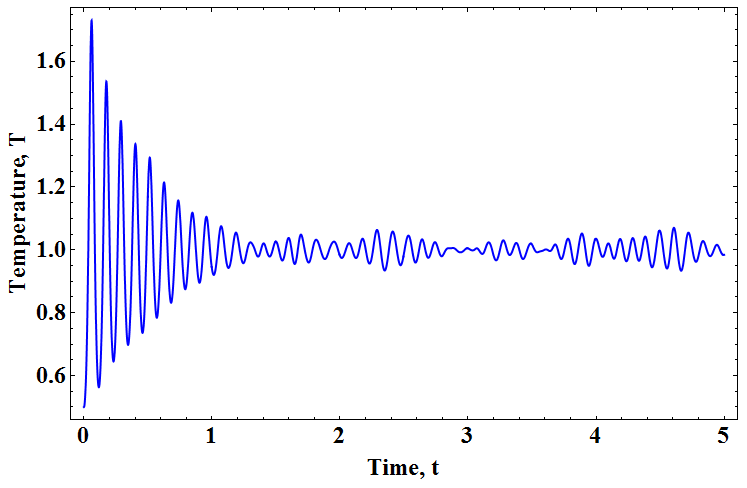
\includegraphics[scale=0.20]{NHres1.png}\qquad}
\subfigure[Energy components]{\label{fig:NHres2}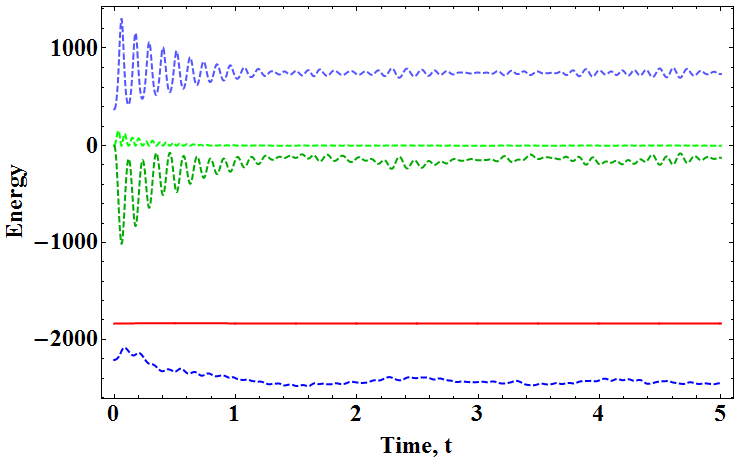
\includegraphics[scale=0.21]{NHres2.png}}
\caption{Plot of instantaneous temperature and energy components of system against time, with $Q = 1.0$ and $T_{eq}=1.0$. The total energy (given in equation (\ref{eqn:hamiltonian})) is the solid red line in (b) - the dashed lines indicate kinetic and potential energy components of the real and artificial system.}
\label{fig:NHres}
\end{figure}

\section{Atmospheric modeling}
\label{sec:atmod}

In this section, we consider a simple atmospheric model using a Lennard-Jones fluid to investigate the presence of fluid droplets and its behaviour, using the algorithm in section \ref{sec:nht}. The motivation of this is to see if the dynamics of the Lennard-Jones fluid is similar to the behaviour of water in the water cycle above the surface of the Earth. In the water cycle, water evaporates from the ground due to heating from solar radiation, and then precipitates as rain droplets at high altitudes, falling down to the surface of the Earth due to gravity. By introducing a (crude) atmospheric model with a Lennard-Jones fluid, we aim to investigate if similar dynamics can be observed.

Figure \ref{fig:atmod} depicts the atmospheric model - it contains three distinct regions, the hot region (for $0<z<h_1$), the intermediate region (for $h_1<z<h_2$) and the cold region (for $z>h_2$). The hot and cold regions are treated as temperature-controlled regions (modelled using Nos\'{e}-Hoover thermostats) at temperatures $T_1$ and $T_2$ respectively (with the obvious constraint $T_1 > T_2$), while the intermediate region is treated as having no temperature control at all (the governing equations of motion are equations (\ref{eqn:motion1}) and (\ref{eqn:motion2}) with $\zeta=0$). We also impose a uniform gravitational field in all regions acting downwards with magnitude $g$ in the atmospheric model. The simulation box (defined by $-\frac{L}{2}<x,y<\frac{L}{2}$ and $z>0$) is subjected to periodic boundary conditions in the $x$ and $y$ directions, and a reflecting boundary is imposed at the $z=0$ plane. We initialize the Lennard-Jones fluid to be placed at the bottom of the simulation box in the hot region.

\begin{figure}[htp]
\centering
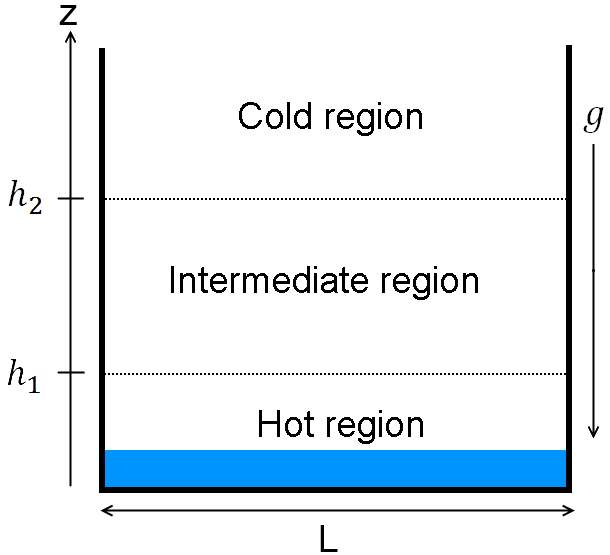
\includegraphics[scale=0.30]{atmod.png}
\caption{Atmospheric model using a Lennard-Jones fluid.}
\label{fig:atmod}
\end{figure}

We have written a program in C++ to simulate the atmospheric model containing a Lennard-Jones fluid. Computations for every time step is parallelized using OpenMP, and graphical output is obtained using the GLUT libraries of OpenGL. Figure \ref{fig:atmodres} shows some sample results obtained, using the parameter set $N = 600$, $\rho = 0.2$, $h_1 = 10$, $h_2 = 30$, $Q_1=Q_2=1.0$, $T_1=2.0$, $T_2=0.2$, $T_0 = 0.5$, $g=0.1$, $\sigma_{coeff}=1.08$ and $\Delta t=0.001$. The parameter $\sigma_{coeff}$ determines the binding length $r_b$ between particles as $r_b = r_{min} \sigma_{coeff} = 2^{1/6} \sigma \sigma_{coeff} = 1.212$ - any particles that are separated by a distance smaller than $r_b$ are classified as being bound together, which is one criteria for a set of particles to be classified as a droplet. Figure \ref{fig:atmodres1} shows the initial setup of the system with the fluid particles initialized to a grid in the hot region, which by heating, causes evaporation of the fluid into the intermediate region, as shown in Figure \ref{fig:atmodres2}. Figure \ref{fig:atmodres3} shows formation of droplets (shown as blue clusters) in the cold region, which then fall down from the cold region as a result of the gravitational force, as seen in Figure \ref{fig:atmodres4}. Once the droplets reach the hot region and hit the $z=0$ boundary, they disperse, and after some time, a sufficient amount of fluid particles evaporates up to the cold region again due to heating, forming droplets which repeat the same process. Hence we can see a rough similarity to the water cycle, that is, a cycle of evaporation and precipitation of the fluid.

\begin{figure}[htp]
\centering
\subfigure[$t = 0$]{\label{fig:atmodres1}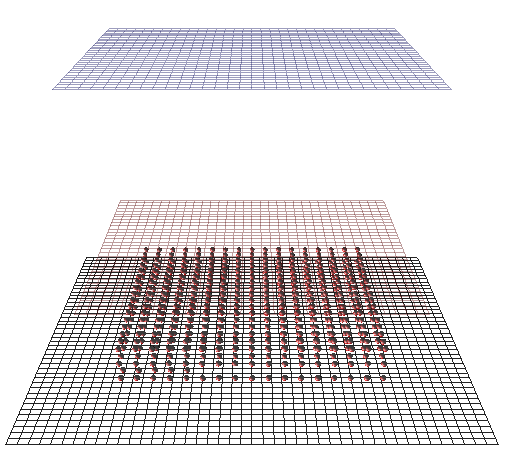
\includegraphics[scale=0.35]{atmodres1.png}\qquad}
\subfigure[$t = 8.9$]{\label{fig:atmodres2}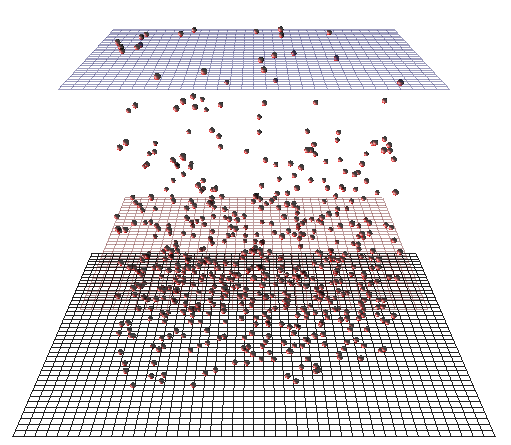
\includegraphics[scale=0.35]{atmodres2.png}}\\
\subfigure[$t = 29.1$]{\label{fig:atmodres3}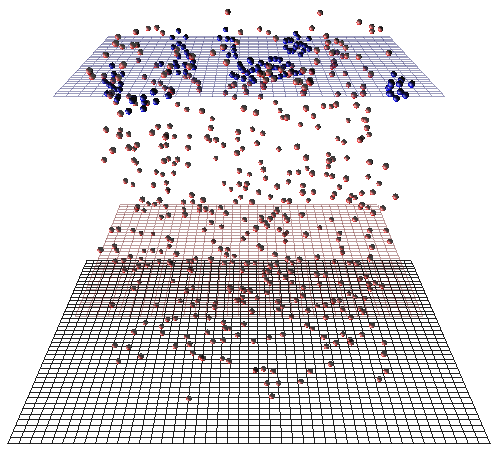
\includegraphics[scale=0.35]{atmodres3.png}\qquad}
\subfigure[$t = 40.5$]{\label{fig:atmodres4}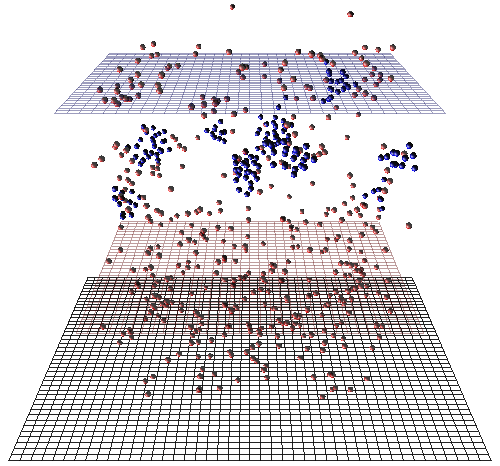
\includegraphics[scale=0.35]{atmodres4.png}}
\caption{Sample graphical output from program showing time-evolution of the Lennard-Jones fluid in the atmospheric model. The black, red and blue grids correspond to the $z=0$, $z=h_1$ and $z=h_2$ planes respectively.
%(a) shows the initial setup of the system with the fluid particles initialized to a grid in the hot region; (b) shows the evaporation of the fluid into the intermediate region as a result of heating; (c) shows formation of droplets (shown as blue clusters) in the cold region; and (d) shows the droplets falling from the cold region as a result of the gravitational force.
}
\label{fig:atmodres}
\end{figure}

Further to this, we can perform some quantitative analysis on the droplets to characterise droplet behaviour over time. Each droplet can be characterized by 3 quantities: the number of particles $n$ in the droplet, its center of mass $\mathbf{r}_{com}$ and the velocity of the center of mass $\mathbf{v}_{com}$. All three quantities evolve with time. Figure \ref{fig:tevol1} shows the time-evolution of two quantities ($n$ and the z-component of $\mathbf{v}_{com}$) for two sample droplets.
\begin{figure}[htp]
\centering
\subfigure[Time-evolution of $n$]{\label{fig:ntevol}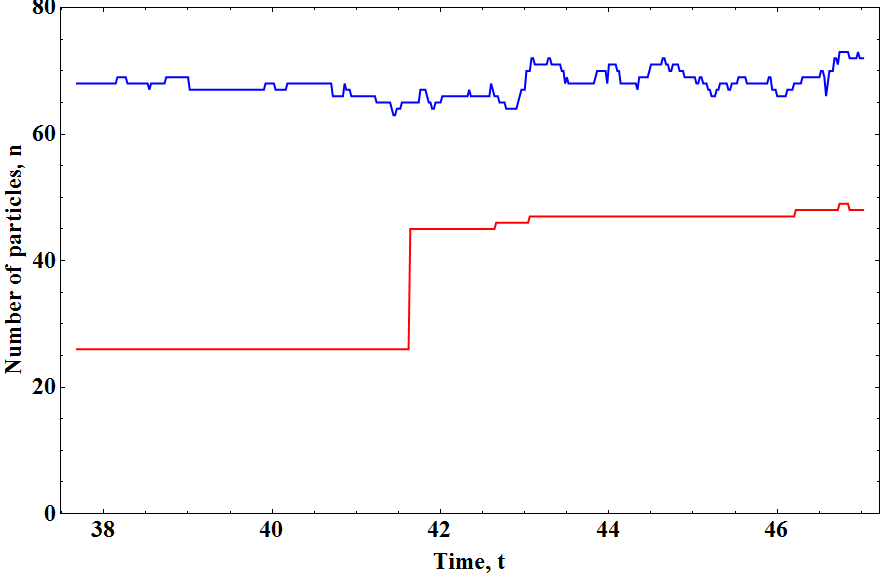
\includegraphics[scale=0.25]{ntevol.png}\qquad}
\subfigure[Time-evolution of z-component of $\mathbf{v}_{com}$]{\label{fig:vcomtevol}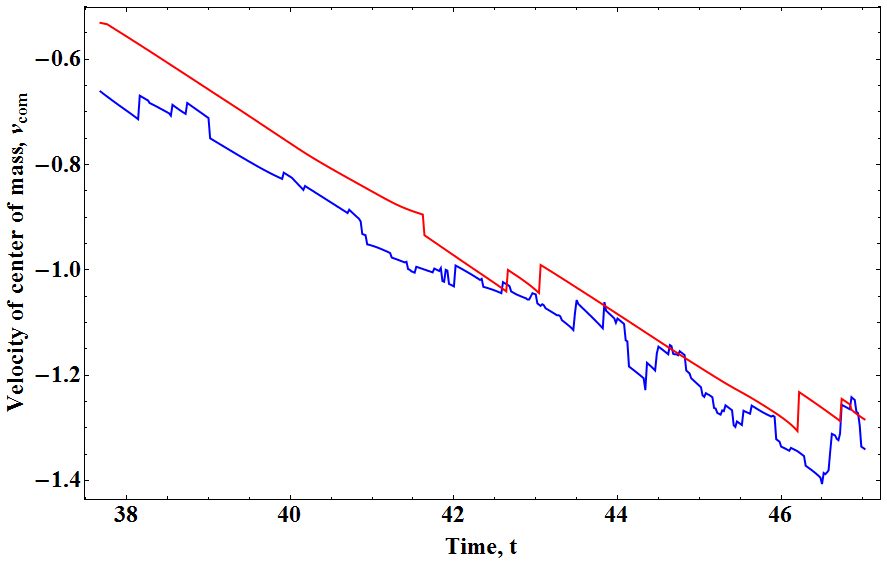
\includegraphics[scale=0.25]{vcomtevol.png}}
\caption{Time-evolution of $n$ and z-component of $\mathbf{v}_{com}$ two sample droplets A (blue) and B (red).}
\label{fig:tevol1}
\end{figure}

From Figure \ref{fig:ntevol}, we can see that $n$ changes slightly over time for droplet A, however, there is a large increase in $n$ for droplet B at around $t=41.5$) before it becomes roughly constant. This large increase can be attributed to droplet B combining with another droplet (of size $\sim 20$). For both droplets, we observe that $n$ does typically fluctuate slightly with time - this is because surrounding particles around the droplet can combine with the droplet, or the particles on the outer surface of the droplet can leave the droplet due to interaction with surrounding particles. Interaction with surrounding particles also does introduce fluctuations in $\mathbf{v}_{com}$. Recalling that the gravitational strength (acting in the -z direction) is $g=0.1$, we would exhibit the z-component of $\mathbf{v}_{com}$ would behave linearly with time, with a gradient of $-g$. Figure \ref{fig:vcomtevol} shows that there is indeed a rough linear trend, but it fluctuates significantly due to interaction with surrounding particles and fluctuations in $n$. Linear fits for each droplet are shown in Figure \ref{fig:tevol2} shows the result of applying a linear least-squares fit to the z-component of $\mathbf{v}_{com}$ for droplets A and B. We find that the overall gradient (i.e. the acceleration) of both droplets are smaller in magnitude than $g$, that is, the droplets fall at a slower rate than would be expected. This can be attributed to a repulsive interaction of the droplet with surrounding particles that are sufficiently close (in terms of the Lennard-Jones potential, this would be for particles which satisfy the criterion $r_{ij} < 2^{1/6}\sigma$) - and since there are typically more particles below the droplet (particles evaporating due to heating) than above, this causes a net force upwards, thus slowing down the droplet.

\begin{figure}[htp]
\centering
\subfigure[Droplet A]{\label{fig:vcom2tevol}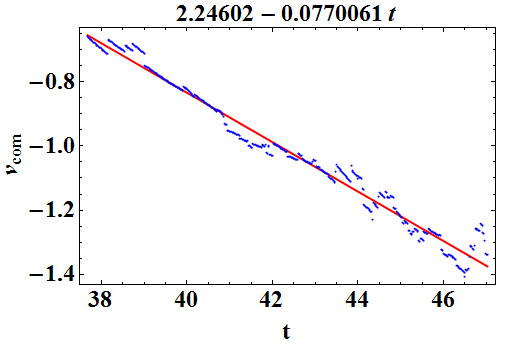
\includegraphics[scale=0.4]{vcom1tevol.png}\qquad}
\subfigure[Droplet B]{\label{fig:vcom2tevol}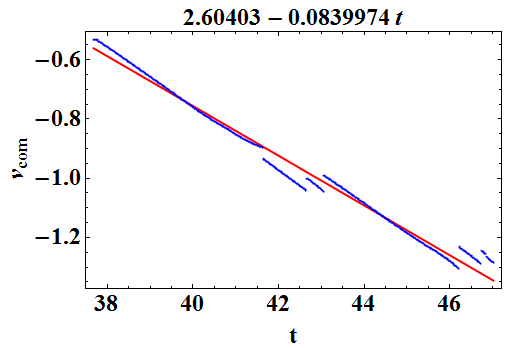
\includegraphics[scale=0.4]{vcom2tevol.png}}
\caption{Linear least-squares fit applied to the z-component of $\mathbf{v}_{com}$ for droplets A and B.}
\label{fig:tevol2}
\end{figure}

\section{Conclusions}
\label{sec:conclusions}

In section \ref{sec:nht}, we have outlined the theory and steps to simulate a Nos\'{e}-Hoover thermostat efficiently. The results obtained from our program have been verified for correctness using standard results. In section \ref{sec:atmod}, we use the theory of section \ref{sec:nht} in order to simulate an atmospheric model using a Lennard-Jones fluid. From our results, we can infer two things regarding this atmospheric model:

\begin{itemize}
\item Qualitatively, droplet formation from a Lennard-Jones fluid does occur under certain conditions, and it occurs repeatedly given sufficient time.
\item Quantitatively, we find that droplets fall at a roughly linear rate due to gravity as expected - however, interaction with surrounding particles causes fluctuations from expected behaviour.
\end{itemize}

In summary, we find that the results for our atmospheric model indicate a rough similarity to the water cycle we find on Earth, in that we observe a cycle of evaporation and precipitation.

\bibliographystyle{unsrt}

\bibliography{References}

\section*{Outlook}

In retrospect, the EXODASS program has been a very valuable experience, primarily from an academic aspect. Through this program, I have gained exposure to molecular dynamics, a field of study that is markedly different from my primary field of research in Australia (quantum computation), but seems almost as interesting. This experience has enabled me to broaden my `toolbox' of techniques for problem-solving, which I will find to be most valuable as I continue my academic life. I also value the friendships and networking developed with the other EXODASS participants, which was a nice break from the routine of working on research almost every day. I would like to thank Prof. Hisashi Okumura for teaching and guiding me in this study of molecular dynamics, and for being incredibly helpful with any problems that I run into. Thanks also to Prof. Hidehiro Sakurai and his staff for organising and running the EXODASS program, without which this experience would not have been possible. Thanks especially to Ms. Hisayo Nagasono for sorting out any and all questions I had about coming to Japan and the paperwork needed - it made the experience a much smoother one.

\end{document}
